\documentclass{article}

\usepackage{graphicx}
\usepackage{subfig}
\usepackage{multirow}
\usepackage{subfigure}


\title{{\bf Supplementary Material:} \\A causal web between chronotype and metabolic health traits}
https://www.overleaf.com/project/605b6416422edc98436c7254
\author{}
\date{}

\begin{document}
\maketitle

Appendix 1: AppendixTable1EpigraphDBIVWresults.xlsx. EpiGraphDB data downloaded to produce Figure 2.

Appendix 2: AppendixTable2StudyCharacteristics.xlsx.
SNP-level information on all 10 studies analyzed needed to reproduce analyses of these 10 studies. to supplementary scatter plots, leave-one-out plots, and Figures 3-5 and supplementary figures.

Appendix 3: AppendixTable3MRAnalysisResults.xlsx. Summary level results for each of the 10 MR analyses, including leave-one-out statistics, MR-Egger statistics, and all MR statistics. Used to produce supplementary scatter plots, leave-one-out plots, and Figures 3-5 and supplementary figures. 

Appendix 4: AppendixTable4ConfounderGraph.xlsx.
Statistics downloaded from EpiGraphDB needed to reproduce figures 6 and 7.


% beer
% diabetes
% bipolar
% omega3
\begin{figure}[htbp]
\begin{subfigure}{\linewidth}
\centering
	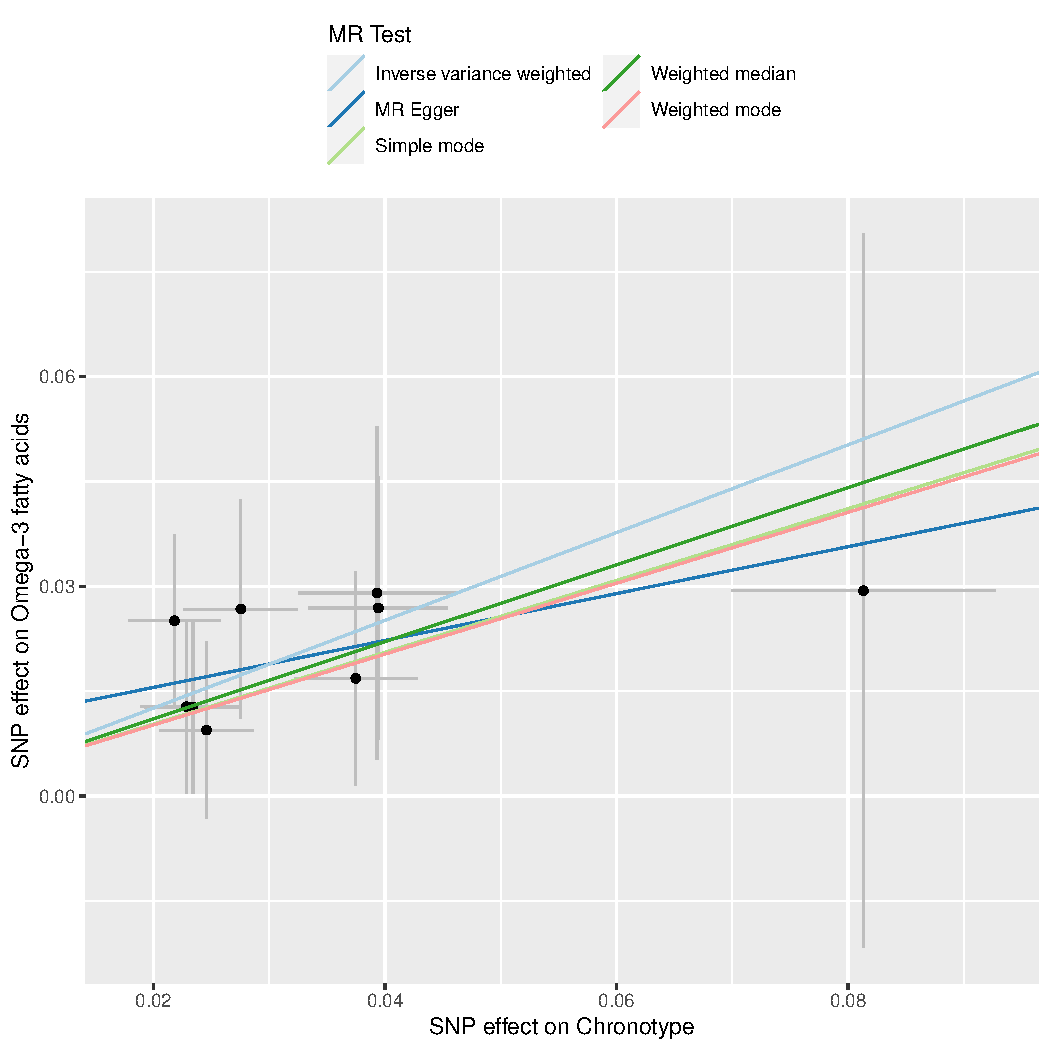
\includegraphics[width=.8\linewidth]{Figs/Analysis2/Chronotype_vs_Omega-3_fatty_acids.Scatterplots.pdf}
\label{omega3Scatter}
\end{subfigure}
\begin{subfigure}{\linewidth}
\centering
	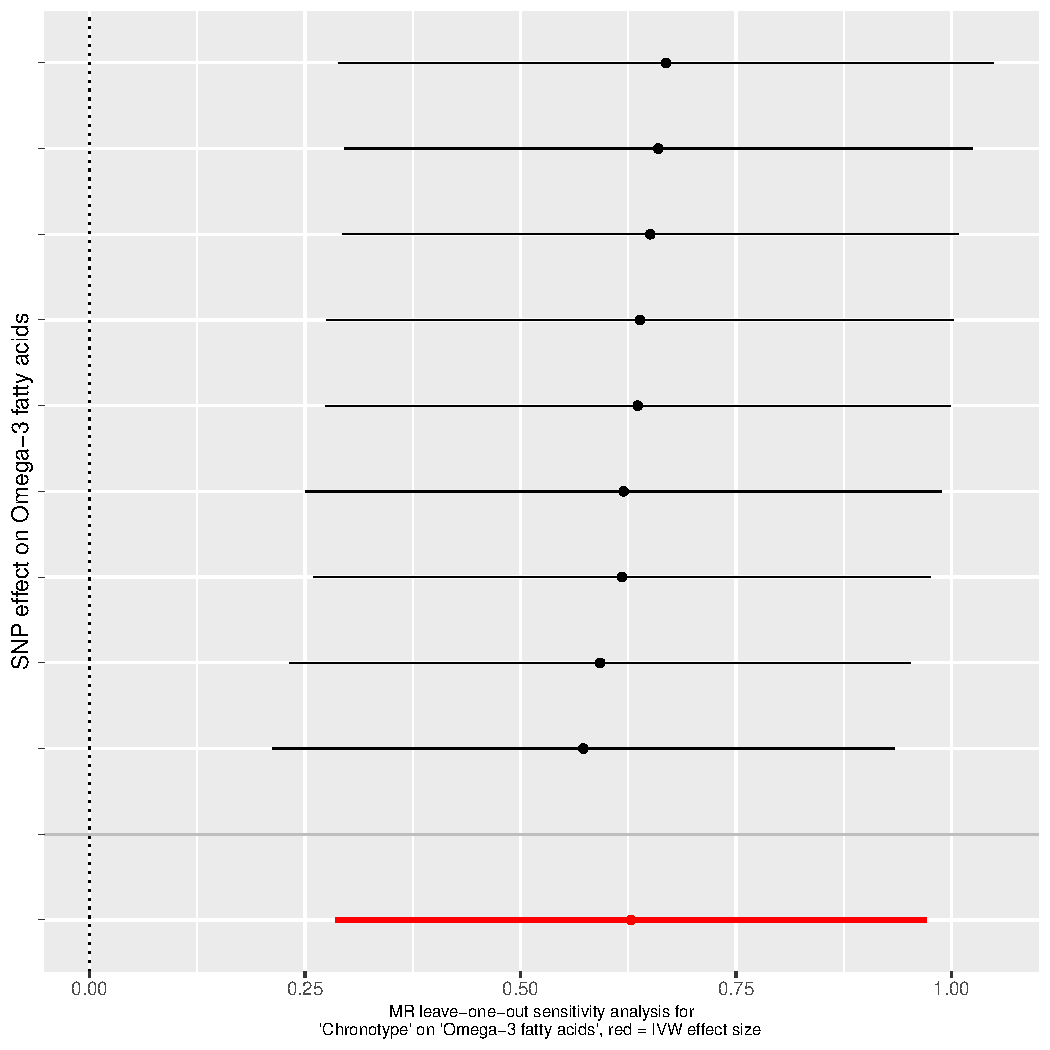
\includegraphics[width=.8\linewidth,keepaspectratio]{Figs/Analysis2/Chronotype_vs_Omega-3_fatty_acids.LOOplots.pdf}
\label{omega3Loo}
\end{subfigure}
\caption{Propensity to an evening chronotype causes increased omega-3 fatty acids. (top) IVW, Weighted median, mode, weighted mode, and Egger regressions shown. Panel (bottom) depicts leave-one-out sensitivity analyses with the IVW method, where the red line indicates the consensus IVW point estimate.}
\label{omega3}
\end{figure}
% triglycerides
\begin{figure}[htbp]
\begin{subfigure}{\linewidth}
\centering
	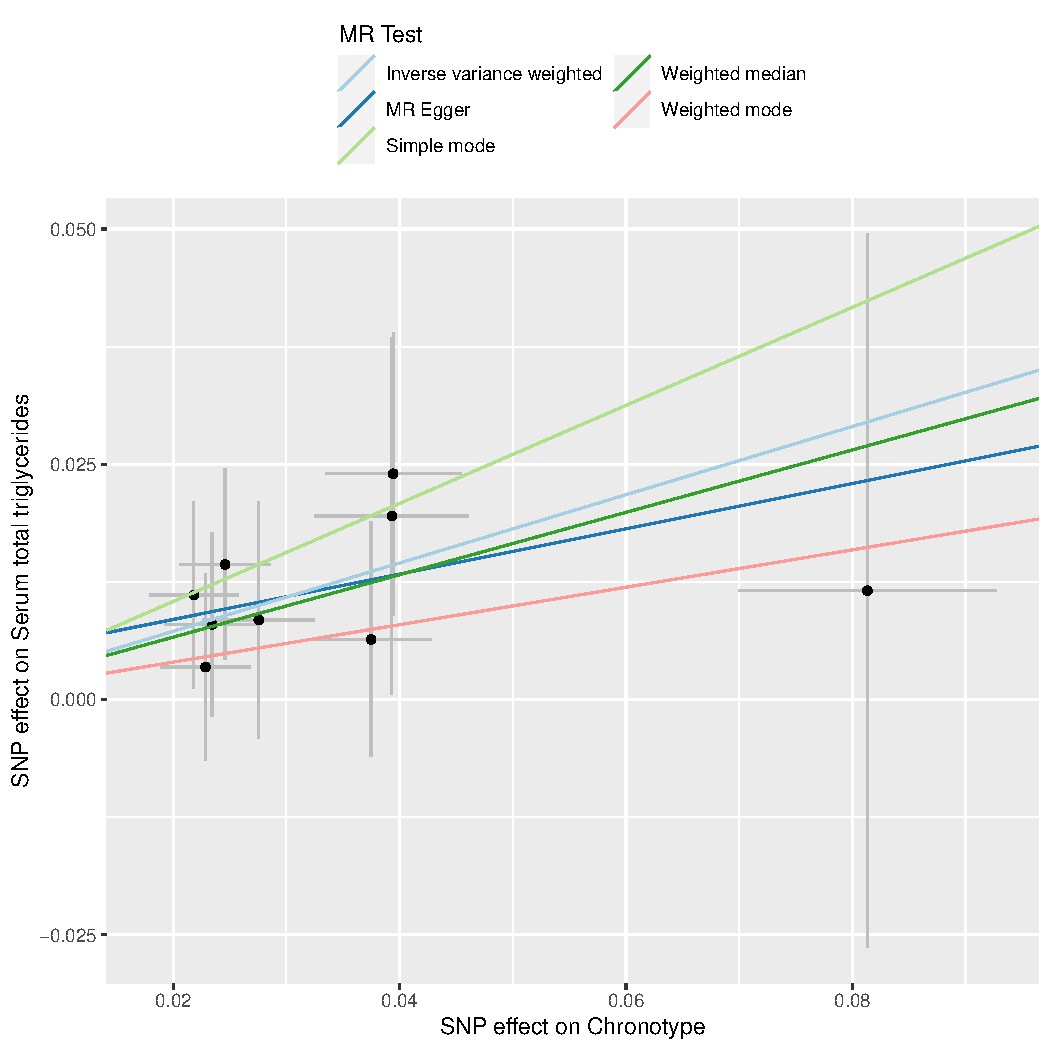
\includegraphics[width=.8\linewidth]{Figs/Analysis2/Chronotype_vs_Serum_total_triglycerides.Scatterplots.pdf}
\label{sttScatter}
\end{subfigure}
\begin{subfigure}{\linewidth}
\centering
	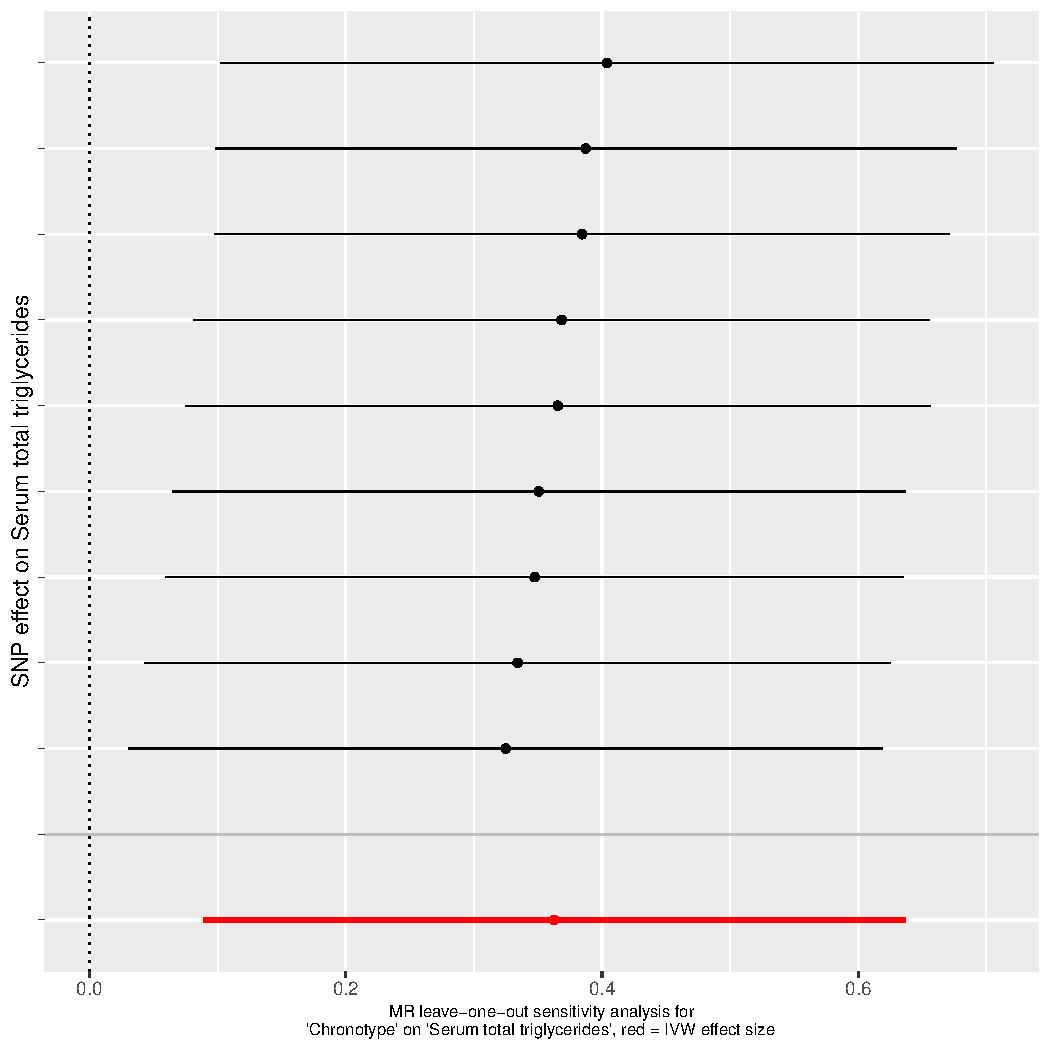
\includegraphics[width=.8\linewidth,keepaspectratio]{Figs/Analysis2/Chronotype_vs_Serum_total_triglycerides.LOOplots.pdf}
\label{sttLoo}
\end{subfigure}
\caption{Propensity to an evening chronotype causes increased serum total triglycerides. (top) IVW, Weighted median, mode, weighted mode, and Egger regressions shown. Panel (bottom) depicts leave-one-out sensitivity analyses with the IVW method, where the red line indicates the consensus IVW point estimate.}
\label{stt}
\end{figure}
%ffa
\begin{figure}[htbp]
\begin{subfigure}{\linewidth}
\centering
	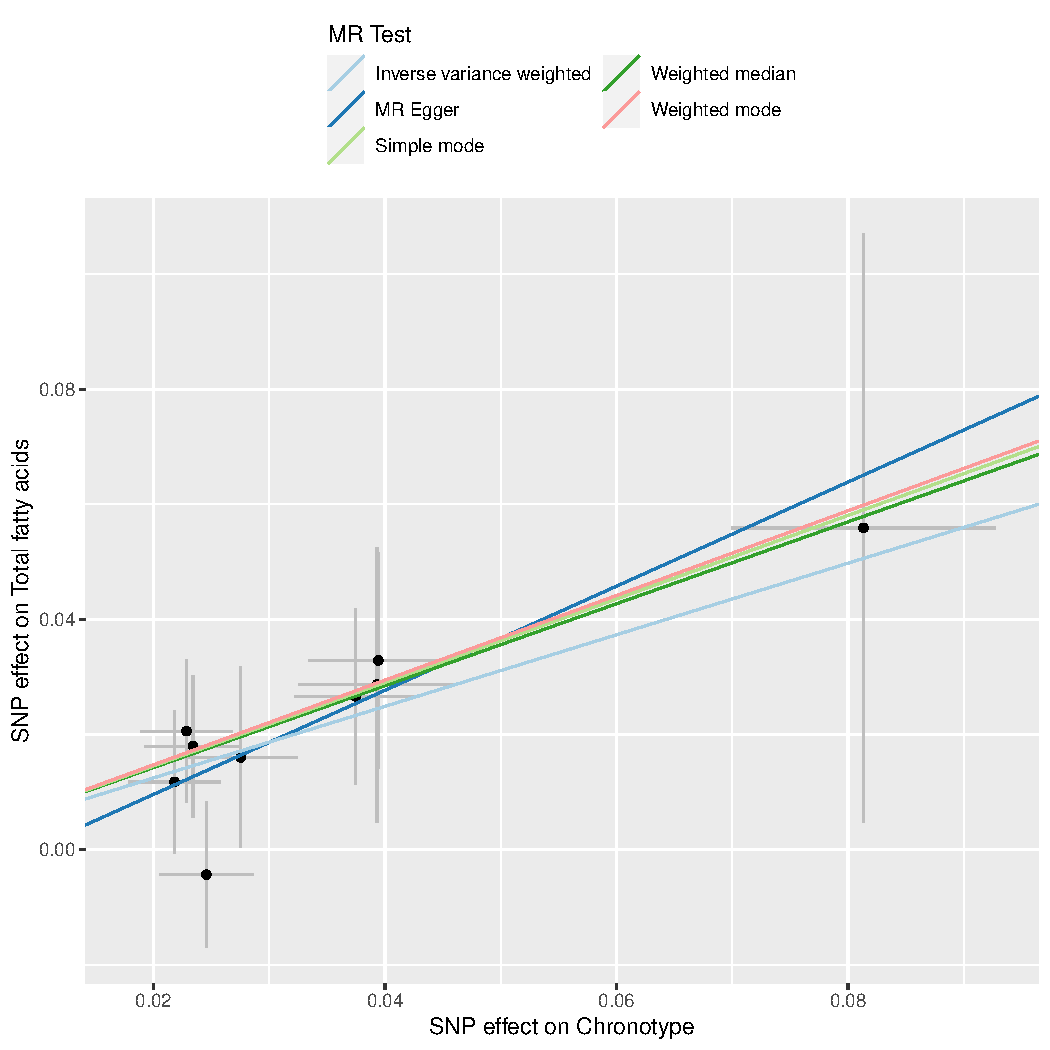
\includegraphics[width=.8\linewidth]{Figs/Analysis2/Chronotype_vs_Total_fatty_acids.Scatterplots.pdf}
\label{ffa3Scatter}
\end{subfigure}
\begin{subfigure}{\linewidth}
\centering
	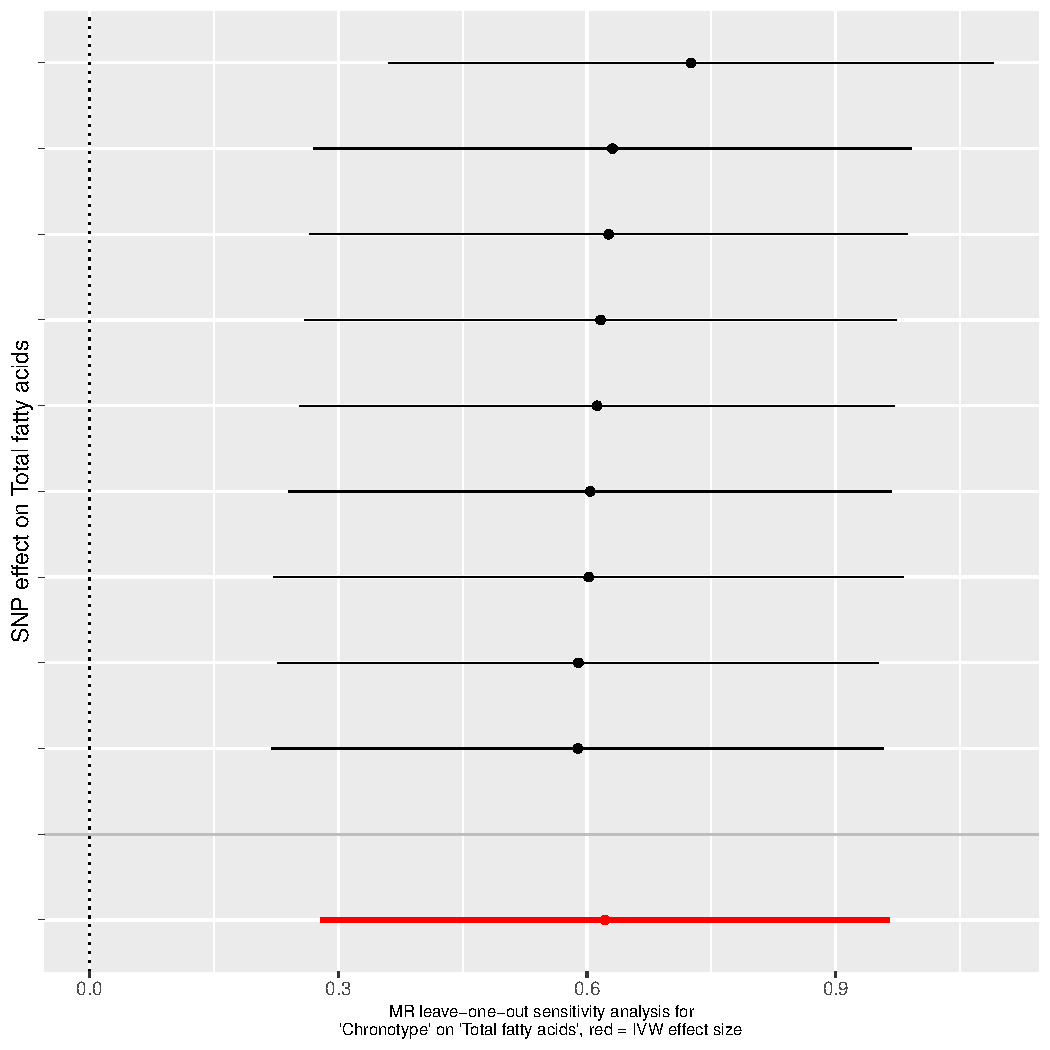
\includegraphics[width=.8\linewidth,keepaspectratio]{Figs/Analysis2/Chronotype_vs_Total_fatty_acids.LOOplots.pdf}
\label{ffaLoo}
\end{subfigure}
\caption{Propensity to an evening chronotype causes increased total fatty acids. (top) IVW, Weighted median, mode, weighted mode, and Egger regressions shown. Panel (bottom) depicts leave-one-out sensitivity analyses with the IVW method, where the red line indicates the consensus IVW point estimate.}
\label{ffa}
\end{figure}
% nicorandil
\begin{figure}[htbp]
\begin{subfigure}{\linewidth}
\centering
	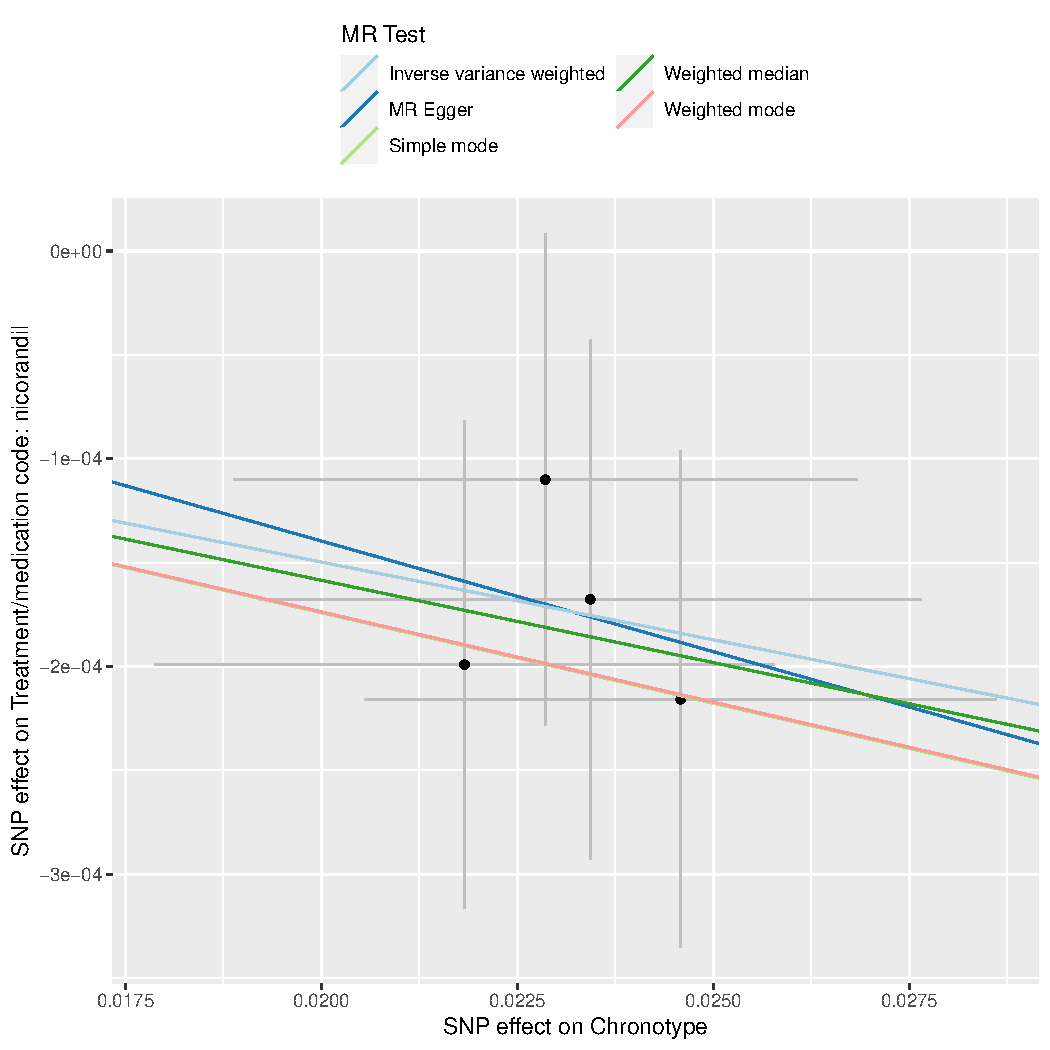
\includegraphics[width=.8\linewidth]{Figs/Analysis2/Chronotype_vs_Treatment_medication_code_nicorandil.Scatterplots.pdf}
\label{nicScatter}
\end{subfigure}
\begin{subfigure}{\linewidth}
\centering
	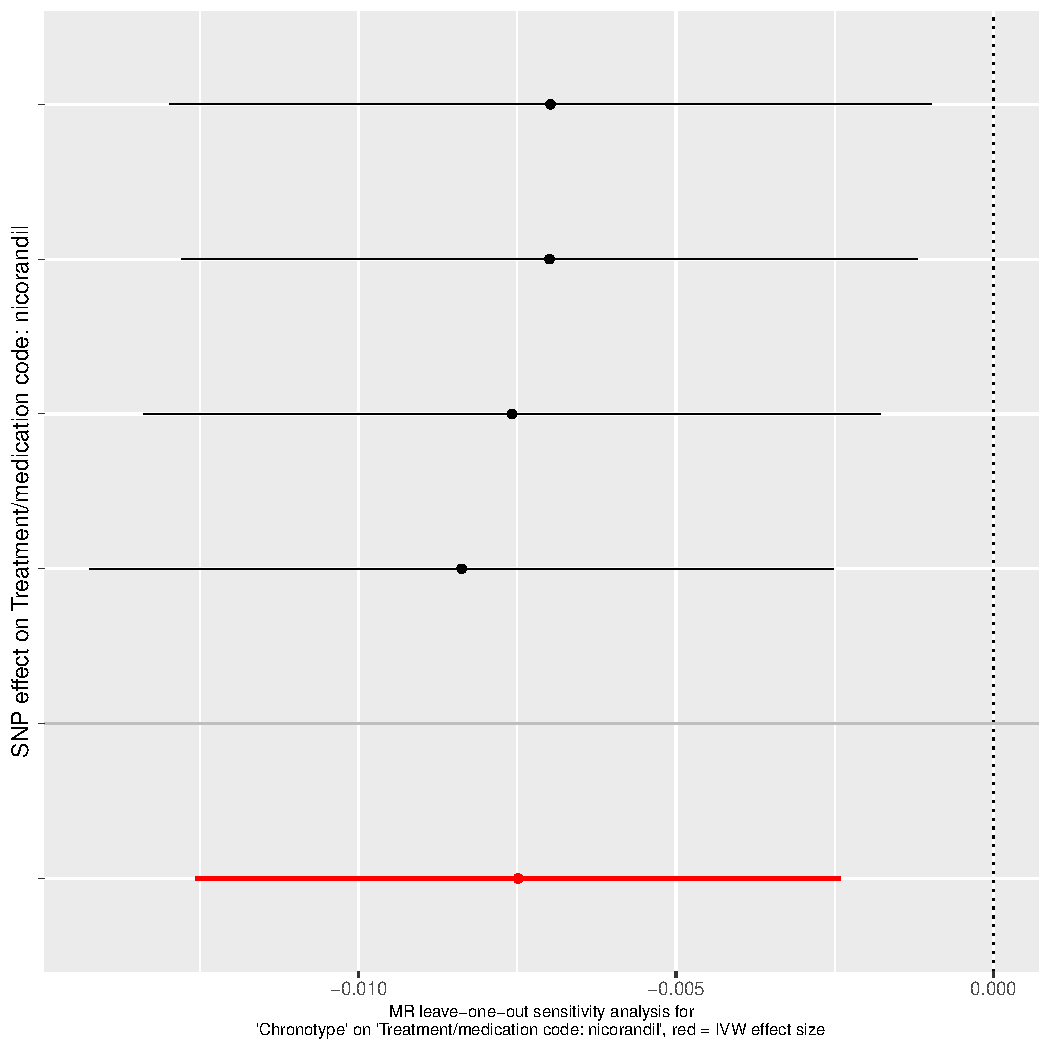
\includegraphics[width=.8\linewidth,keepaspectratio]{Figs/Analysis2/Chronotype_vs_Treatment_medication_code_nicorandil.LOOplots.pdf}
\label{nicLoo}
\end{subfigure}
\caption{Propensity to an evening chronotype causes decreased likelihood of treatment with nicorandil. (top) IVW, Weighted median, mode, weighted mode, and Egger regressions shown. Panel (bottom) depicts leave-one-out sensitivity analyses with the IVW method, where the red line indicates the consensus IVW point estimate.}
\label{nic}
\end{figure}
% lethargy
\begin{figure}[htbp]
\begin{subfigure}{\linewidth}
\centering
	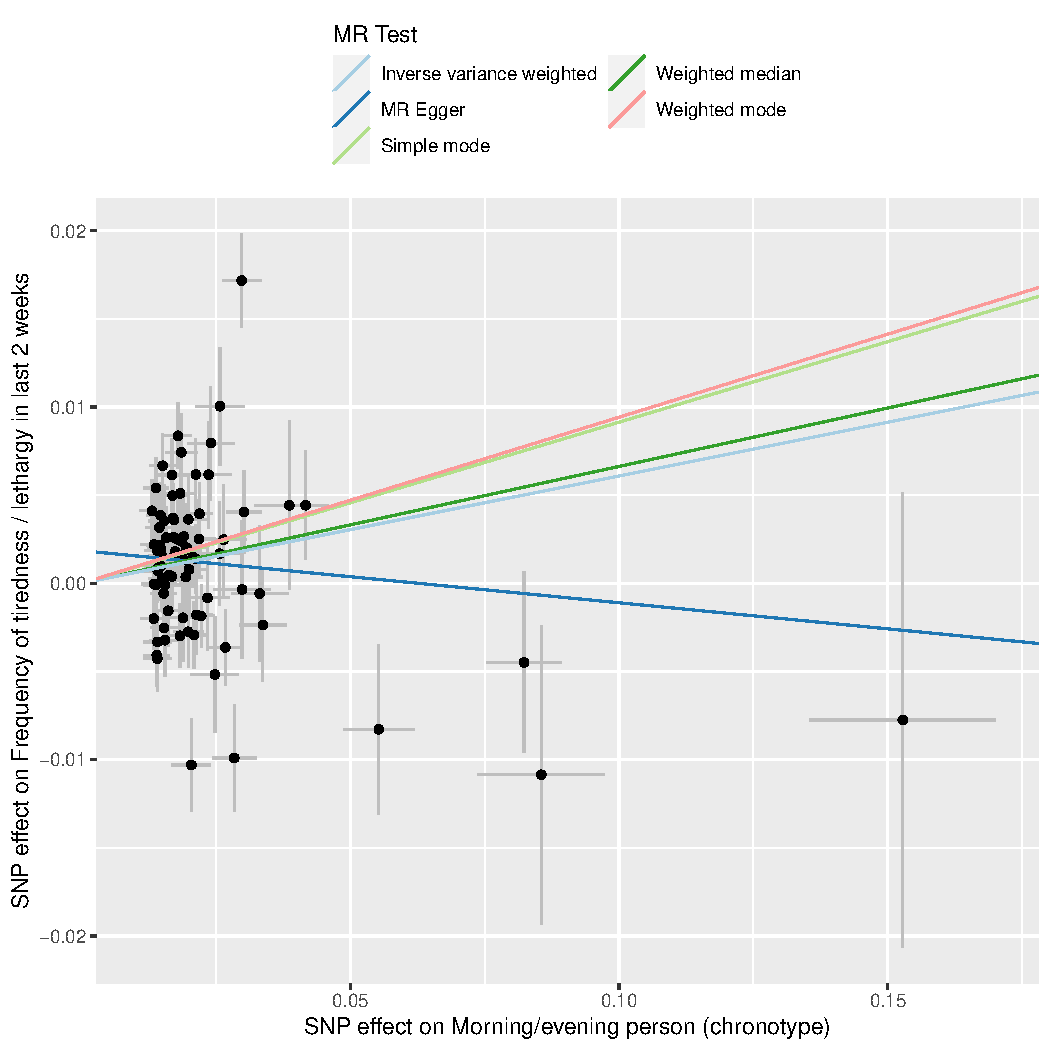
\includegraphics[width=.8\linewidth]{Figs/Analysis2/Morning_evening_person_(chronotype)_vs_Frequency_of_tiredness___lethargy_in_last_2_weeks.Scatterplots.pdf}
\label{lethargyScatter}
\end{subfigure}
\begin{subfigure}{\linewidth}
\centering
	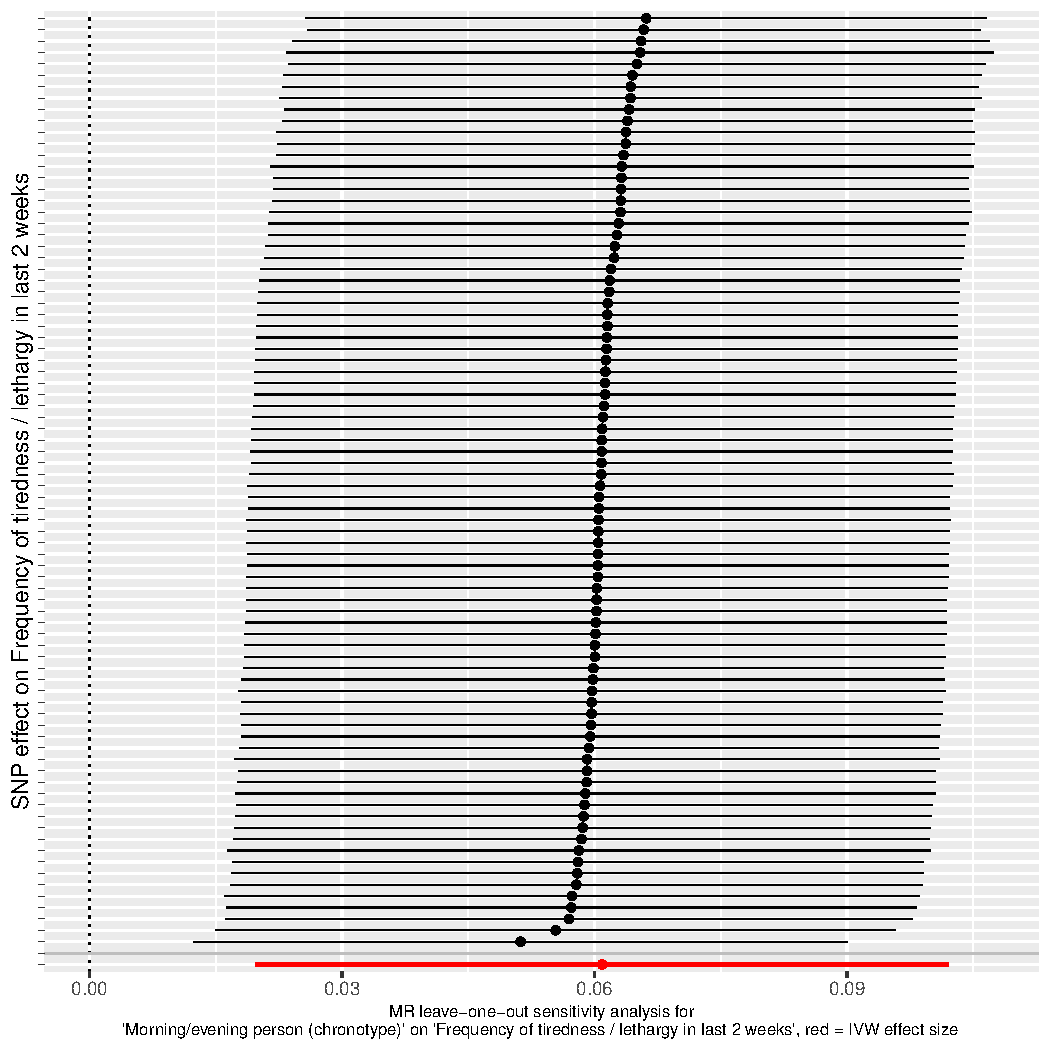
\includegraphics[width=.8\linewidth,keepaspectratio]{Figs/Analysis2/Morning_evening_person_(chronotype)_vs_Frequency_of_tiredness___lethargy_in_last_2_weeks.LOOplots.pdf}
\label{lethargyLoo}
\end{subfigure}
\caption{Propensity to an evening chronotype causes increases in self-reported lethargy in the last two weeks. (top) IVW, Weighted median, mode, weighted mode, and Egger regressions shown. Panel (bottom) depicts leave-one-out sensitivity analyses with the IVW method, where the red line indicates the consensus IVW point estimate.}
\label{lethargy}
\end{figure}

% test
% lethargy
\begin{figure}[htbp]
\begin{subfigure}{\linewidth}
\centering
	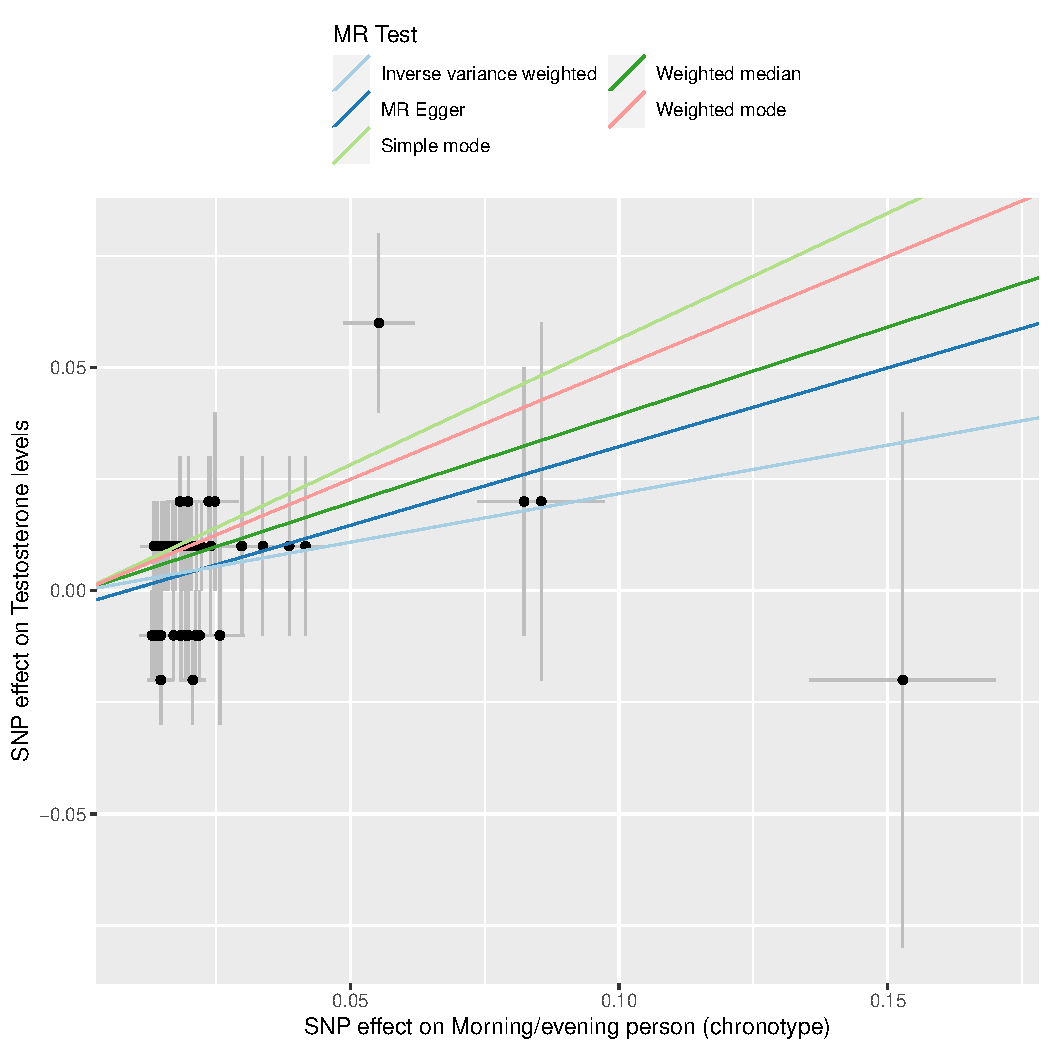
\includegraphics[width=.8\linewidth]{Figs/Analysis2/Morning_evening_person_(chronotype)_vs_Testosterone_levels.Scatterplots.pdf}
\label{testScatter}
\end{subfigure}
\begin{subfigure}{\linewidth}
\centering
	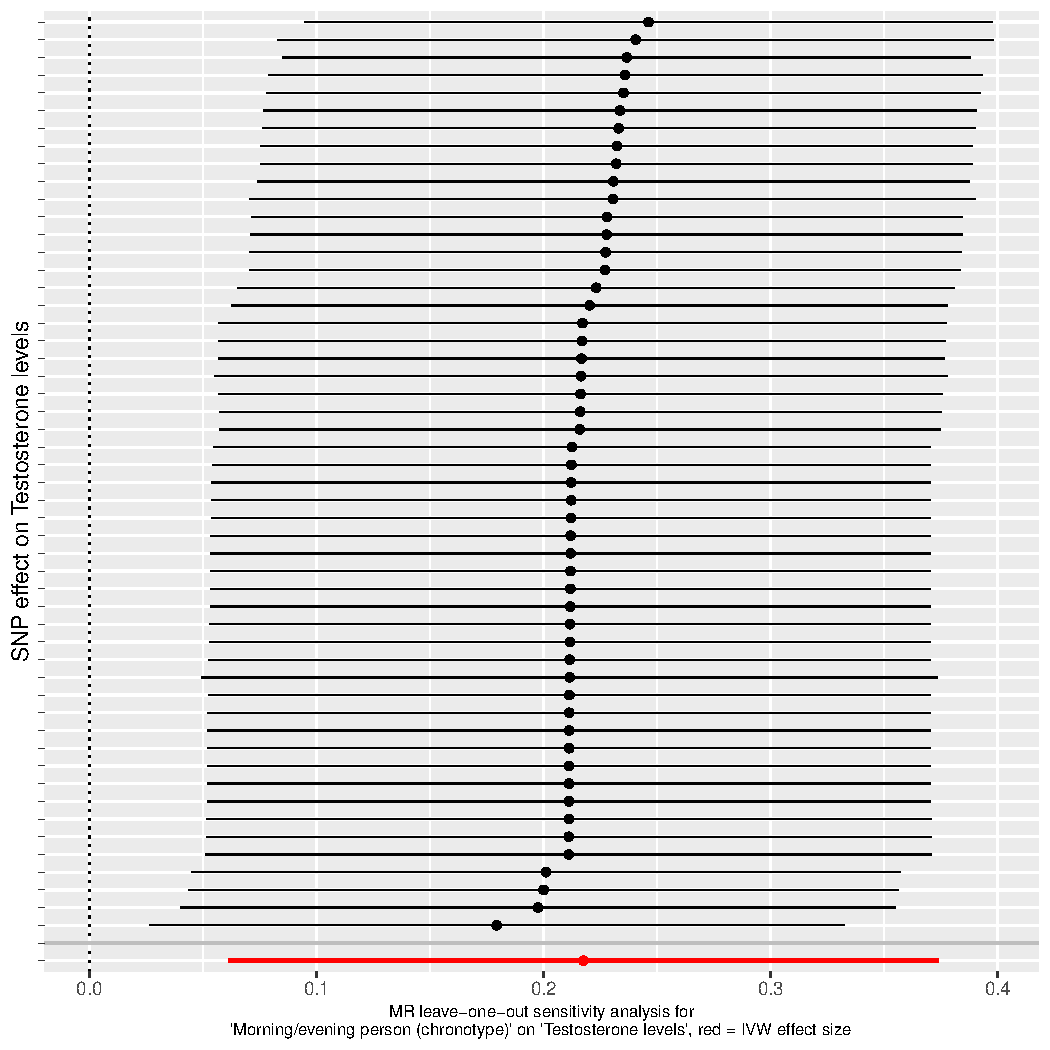
\includegraphics[width=.8\linewidth,keepaspectratio]{Figs/Analysis2/Morning_evening_person_(chronotype)_vs_Testosterone_levels.LOOplots.pdf}
\label{testLoo}
\end{subfigure}
\caption{Propensity to an evening chronotype causes increases in serum testosterone. (top) IVW, Weighted median, mode, weighted mode, and Egger regressions shown. Panel (bottom) depicts leave-one-out sensitivity analyses with the IVW method, where the red line indicates the consensus IVW point estimate.}
\label{test}
\end{figure}
% waking
\begin{figure}[htbp]
\begin{subfigure}{\linewidth}
\centering
	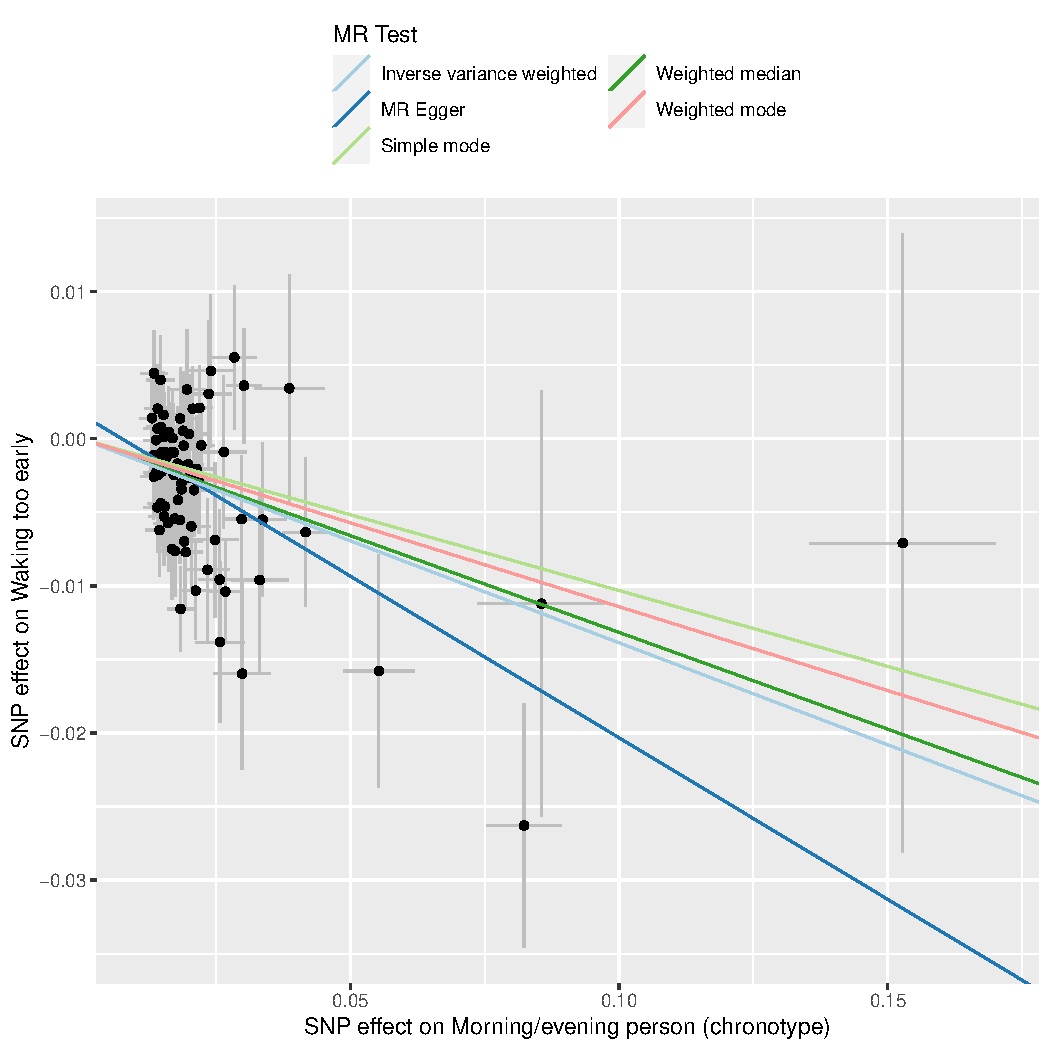
\includegraphics[width=.8\linewidth]{Figs/Analysis2/Morning_evening_person_(chronotype)_vs_Waking_too_early.Scatterplots.pdf}
\label{wakeScatter}
\end{subfigure}
\begin{subfigure}{\linewidth}
\centering
	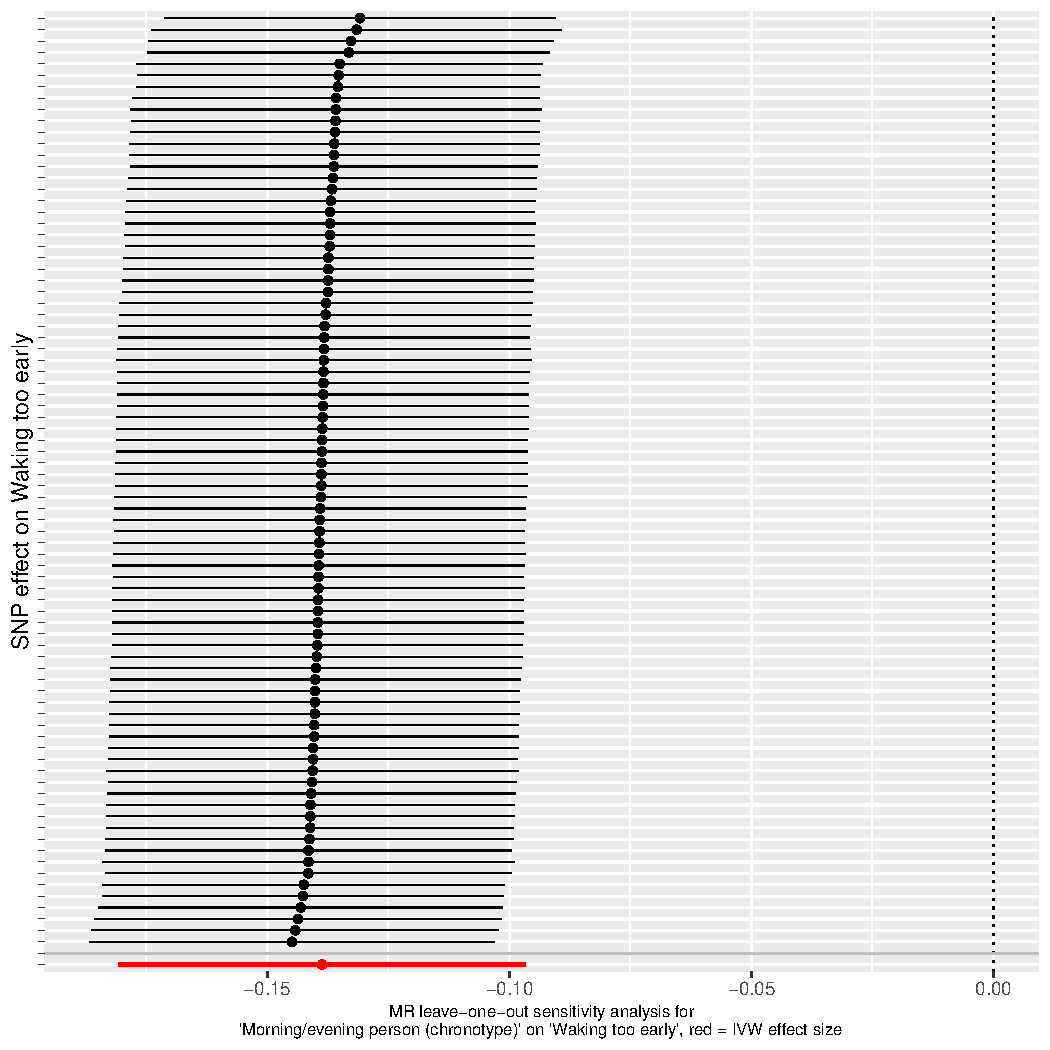
\includegraphics[width=.8\linewidth,keepaspectratio]{Figs/Analysis2/Morning_evening_person_(chronotype)_vs_Waking_too_early.LOOplots.pdf}
\label{wakeLoo}
\end{subfigure}
\caption{Propensity to an evening chronotype causes decrease in odds of waking early. (top) IVW, Weighted median, mode, weighted mode, and Egger regressions shown. Panel (bottom) depicts leave-one-out sensitivity analyses with the IVW method, where the red line indicates the consensus IVW point estimate.}
\label{wake}
\end{figure}



\end{document}